% =====================================================================================
% fig_pareto.tex: accuracy of the rules vs size of the explanations (Q2).
%
% What the experiment tests: every self-explainable model gives, for each prediction, a
%   rule-based explanation. A useful model is both accurate AS RULES (not only as a
%   network) and short to read. This figure places each model of table_interp.tex in
%   that plane, one point per (model, fold), per dataset.
% Plot: one panel per dataset (Mutagenicity, PROTEINS, BAMultiShapes; others in the
%   appendix). x = explanation size per prediction (trunk bits, log scale; table_interp
%   "Bits"), y = rule-model test accuracy. Markers: classic LogiX-GIN (± sum), graph,
%   NMP, NMP+QAT (and the K variants of table_num_prototypes.tex as smaller markers);
%   one dot per fold, the model's mean as a larger marker with std bars. Horizontal line:
%   the GIN teacher's mean test accuracy. Competitors as extra markers if they define an
%   explanation size.
% What it shows: the trade-off between faithful accuracy and explanation length; that
%   classic LogiX-GIN rules are short but inaccurate (fidelity ~65-80%), graph-level
%   prototypes are accurate but long (~1000 bits: every bit of the pooled embedding),
%   NMP+QAT sits at the knee (expected from the preliminary numbers: Mutagenicity 77% at
%   ~43 evidence bits vs NMP 67% at ~21 bits).
% What it does not show: whether the trunk bits are themselves readable (layers 1-2 need
%   ~10-14 literals each, table_hoyer.tex); the network accuracy (table_main.tex); human
%   usefulness. Size is the evidence (input-dependent literals only; constant head
%   literals are a bias), config size: evidence; the plain count is in the appendix.
% Data: results_final/<exp>/<dataset>/<model>/fold<k>/interp.json
%   (test_interp_logic_acc, test_interp_expl_bits_evidence_mean) of the final E1 experiment.
% GENERATED BY: python plot_paper.py pareto   (sources: configs/paper_figures.yaml, code:
%   utils/paper_figures.py, branch feat/paper-figures). "preliminary: true" in the config
%   stamps PRELIMINARY on the figure; set it to false only when every source is final.
% STATUS: PRELIMINARY version drawn 2026-10-21 (sum_ablation / sum_ablation_ctrl / qat_nmp*, pre head-fix). Final after E1.
% TODO:
%   [ ] after E1 final + evidence-only size; style with the dataviz palette, colour-blind safe.
% =====================================================================================
\begin{figure*}[t]
  \centering
  \IfFileExists{figures/fig_pareto.pdf}{%
    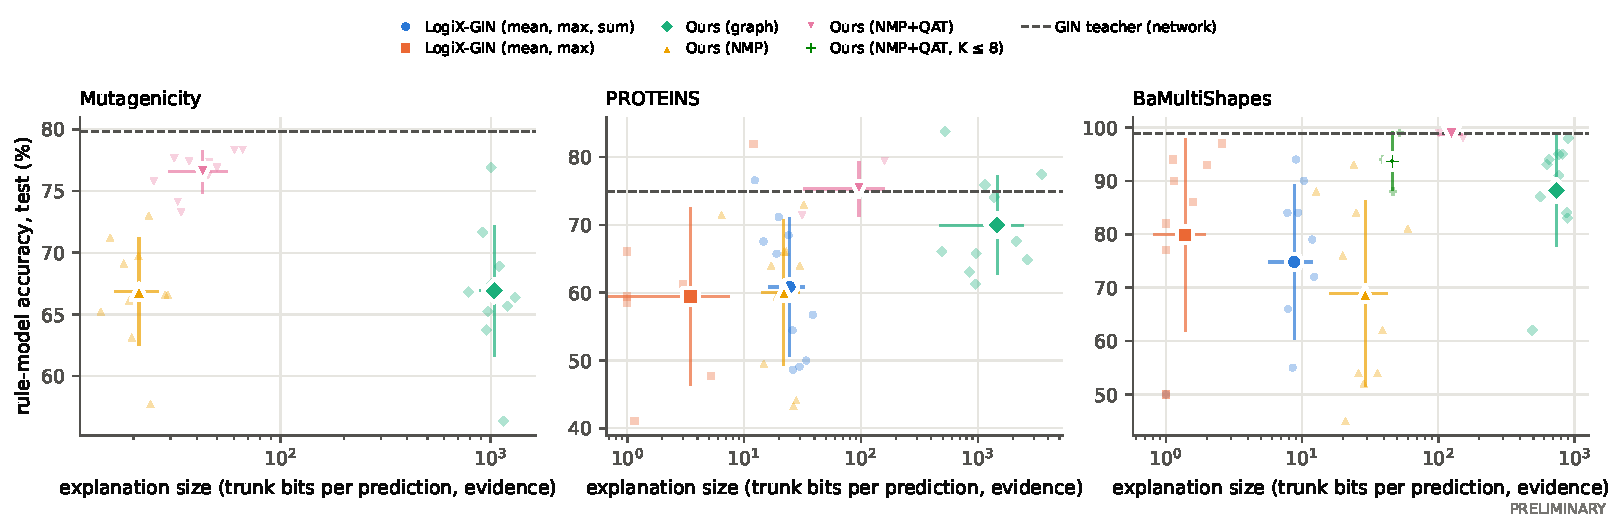
\includegraphics[width=\textwidth]{figures/fig_pareto.pdf}%
  }{\fbox{\parbox[c][4cm]{0.95\textwidth}{\centering\todo{fig\_pareto.pdf: rule-model accuracy vs explanation size}}}}
  \caption{Accuracy of the rule model against the size of its explanations (trunk bits
    per prediction, log scale), test split, one small dot per fold and the mean $\pm$ std
    per model. Dashed line: \teacher{}. Up and to the left is better.}
  \label{fig:pareto}
\end{figure*}
